\documentclass[a4paper,twoside]{article}
\usepackage{a4wide,graphicx,fancyhdr,amsmath,amssymb,csquotes,caption, subcaption, url,hyperref}
\usepackage[english]{babel}
\usepackage[backend=biber, maxbibnames=10]{biblatex}
\usepackage[colorinlistoftodos]{todonotes}
\usepackage{regexpatch}
%\tracingxpatches%for debugging
\makeatletter
\xpatchcmd{\@todo}{\setkeys{todonotes}{#1}}{\setkeys{todonotes}{inline,#1}}{}{}
\NewBibliographyString{artno}
\DefineBibliographyStrings{english}{artno = {Art\adddotspace No\adddot}}

\DeclareFieldFormat[article,periodical]{eid}{\bibstring{artno}\addabbrvspace #1}

\addbibresource{resources.bib}
%
%----------------------- Macros and Definitions --------------------------

\setlength\headheight{20pt}
\addtolength\topmargin{-10pt}
\addtolength\footskip{20pt}

\fancypagestyle{plain}{%
\fancyhf{}
\fancyhead[LO,RE]{\sffamily\bfseries\large }
\fancyhead[RO,LE]{\sffamily\bfseries\large 2IMC0 Preparation Graduation Project ES}
\fancyfoot[LO,RE]{\sffamily\bfseries\large department of mathematics and computer science}
\fancyfoot[RO,LE]{\sffamily\bfseries\thepage}
\renewcommand{\headrulewidth}{0pt}
\renewcommand{\footrulewidth}{0pt}
}

\pagestyle{fancy}
\fancyhf{}
\fancyhead[RO,LE]{\sffamily\bfseries\large }
\fancyhead[LO,RE]{\sffamily\bfseries\large 2IMC0 Preparation Graduation Project ES}
\fancyfoot[LO,RE]{\sffamily\bfseries\large department of mathematics and computer science}
\fancyfoot[RO,LE]{\sffamily\bfseries\thepage}
\renewcommand{\headrulewidth}{1pt}
\renewcommand{\footrulewidth}{0pt}

%--------------------------------- Text ----------------------------------

\begin{document}
	\pagenumbering{roman}
	\begin{titlepage}

\newcommand{\HRule}{\rule{\linewidth}{0.5mm}} % Defines a new command for the horizontal lines, change thickness here

\center % Center everything on the page
 
%----------------------------------------------------------------------------------------
%	HEADING SECTIONS
%----------------------------------------------------------------------------------------

\includegraphics[width=0.55\textwidth]{images/tuelogonew.png}\\[0.7cm]
\textsc{\LARGE Eindhoven University of Technology}\\[2.5cm] % Name of your university/college

%----------------------------------------------------------------------------------------
%	TITLE SECTION
%----------------------------------------------------------------------------------------

\HRule \\[0.4cm]
{ \huge \bfseries Preparation Graduation Project ES}\\[0.4cm] % Title of your document
2IMC05
\HRule \\[2cm]
 
%----------------------------------------------------------------------------------------
%	AUTHOR SECTION
%----------------------------------------------------------------------------------------

\begin{minipage}[t]{0.5\textwidth}
\begin{flushleft} \large
\emph{Author:}\\
Stephan P.O \textsc{Oostveen}\\
\end{flushleft}
\end{minipage}
~
\begin{minipage}[t]{0.39\textwidth}
\begin{flushright} \large
\emph{Graduation supervisor:} \\ 
Pieter J.L \textsc{Cuijpers}\\  % Supervisor's Name
\end{flushright}
\end{minipage}\\[4cm]

% If you don't want a supervisor, uncomment the two lines below and remove the section above
%\Large \emph{Author:}\\
%John \textsc{Smith}\\[3cm] % Your name

%----------------------------------------------------------------------------------------
%	DATE SECTION
%----------------------------------------------------------------------------------------
{\large \today}\\[3cm] % Date, change the \today to a set date if you want to be precise

%----------------------------------------------------------------------------------------

\vfill % Fill the rest of the page with whitespace

\end{titlepage}
	\tableofcontents
	\newpage
	\pagenumbering{arabic}
	\section{Introduction}
\label{sec:introduction}
Lightyear designs and develops solar electric vehicles (SEVs), these are highly efficient battery electric vehicles that can charge their batteries using an integrated solar panel. The following factors play a role in a vehicle's efficiency: Aerodynamic drag, friction losses from tires, cabin heating and cooling, drivetrain losses, static energy consumption. Lightyear seeks to design a vehicle that minimizes these losses as a reduction in energy consumption has a snowball effect on vehicle efficiency. For example, a lower aerodynamic drag enables the use of a smaller battery pack while maintaining the same range, reducing the vehicle weight, resulting in less friction losses from the tires etc. In the end yielding a very efficient vehicle that can charge at any time using the power of the sun. Lightyear is constantly searching for solutions which improve vehicle efficiency, one key aspect which can be optimized is the electrical/electronic architecture.

\subsection{Current and future automotive architectures}
\label{sec:automotive-arch}
Modern vehicles are mostly electrically/electronically controlled, ranging from basic functionality such as acceleration (throttle pedal) and lighting to more advanced features such as ride height control and Autonomous Emergency Braking System. The number of electrically/electronically controlled features has grown over time by adding several electronic control units (ECUs) per feature to an already existing decentralized control architecture. This means that multiple ECUs need to communicate in order to achieve a certain function. As a result modern vehicles can contain more than 100 ECUs~\cite{bandur2021making} and several communication networks. This has several drawbacks: increased communication load on the in-vehicle network(s), increased cost due to the large number of ECUs and large wiring harness, increased software complexity, more software variants, higher maintenance costs and reduced reliability~\cite{bandur2021making}. An example of such a decentralized architecture is shown in Figure~\ref{fig:functional-arch}, the blue rectangles represent ECUs, ECUs that are part of a single function or domain (body control, drivetrain etc) are connected to each other with an automotive network such as LIN or CAN. The functions or domains work together by means of a gateway (red rectangle) which bridges or translates messages to and from the different networks. Sometimes certain ECUs are also connected to more than one network for practical reasons such as the Steering column ECU in the example.

\begin{figure}[htb]
    \centering
    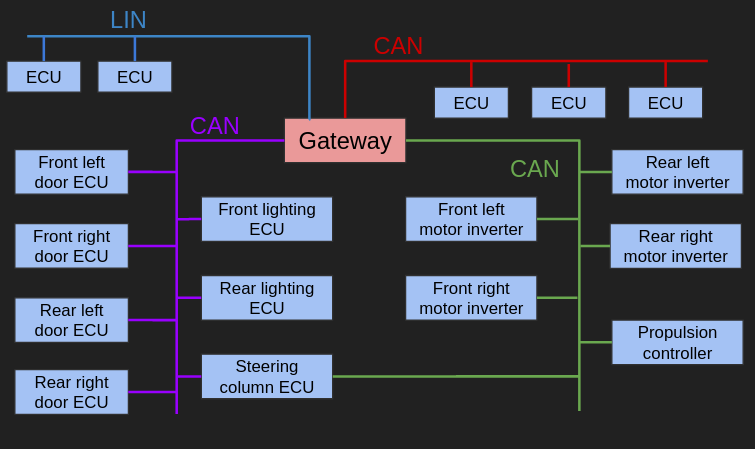
\includegraphics[width=\textwidth]{images/functional-arch.png}
    \caption{Example of an automotive decentralized control architecture}
    \label{fig:functional-arch}
\end{figure}

The automotive industry has recognized these issues and is moving towards a centralized control architecture with one large ECU per physical zone, called a zonal architecture~\cite{ashjaei2021time}. Instead of having many small ECUs performing only one part of a function there will be one central ECU responsible for all the control functions and a few large ECUs (zone ECUs) strategically placed in the car executing the commands of the central controller. To reduce complexity, weight and cost even more the zone ECUs are networked through a single high bandwidth, low latency network instead of the multiple low bandwidth networks running through a vehicle nowadays. The zone ECUs can act as a bridge for legacy networks used by legacy components in the physical neighbourhood. An example is depicted in Figure~\ref{fig:zonal-arch}.

In the zonal architecture the zone ECUs and central controller are connected through a high bandwidth low latency network, automotive Ethernet together with Time Sensitive Networking (TSN) have been chosen as the key networking technologies. The choice for automotive Ethernet is supported by the work of the Time Sensitive Networking (TSN) Task Group of the IEEE 802.1 Working Group, which allow real-time communication over IEEE 802.3 (Ethernet) networks~\cite{klaus2019zonal}. Other relevant factors are the high bandwidth capabilities relative to traditional networking technologies such as CAN and FlexRay, Internet Protocol (IP) based end to end communication support, automotive specific physical layer standards for various data rates and standardization by the IEEE~\cite{ashjaei2021time}.

Figure~\ref{fig:zonal-arch} represents the same vehicle as in Figure~\ref{fig:functional-arch} with a zonal architecture. The number of ECUs, including gateway, is reduced from 18 in the decentralized architecture to 11 in the zonal architecture. This reduction has been achieved by consolidating several ECUs into the zone ECUs, reducing mass. The number of networks has stayed the same, three CAN networks and one LIN network in the decentralized control architecture versus 3 CAN networks and one Ethernet network in the zonal architecture. But crucially the physical wiring loom has been simplified in the zonal architecture as there is only one network cable spanning the entire vehicle length. This simplification reduces weight, since there is only one cable going from the back to the front instead of two or more. Additionally, the shorter sub-wire harnesses can be manufactured automatically, reducing costs.

\begin{figure}[htb]
    \centering
    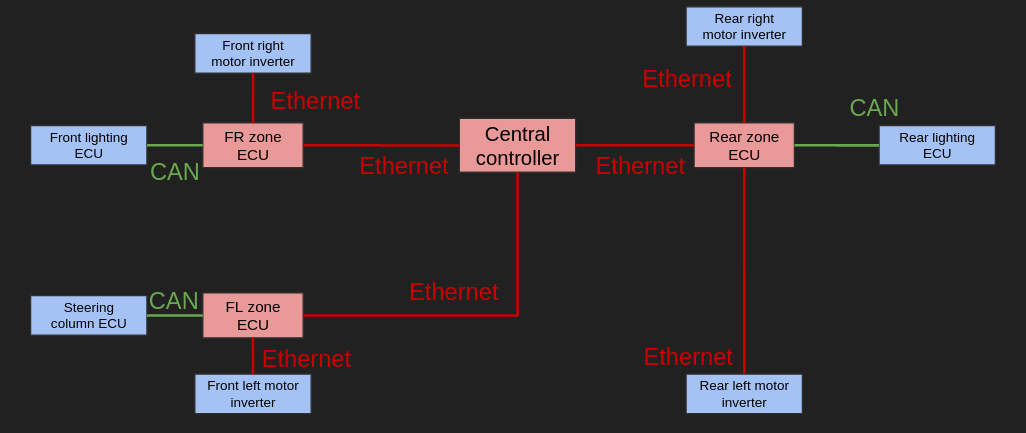
\includegraphics[width=\textwidth]{images/zone-arch.png}
    \caption{Example of an automotive zonal architecture}
    \label{fig:zonal-arch}
\end{figure}

\subsection{Real-time communication over Ethernet}
Some electrically/electronically features in a vehicle pose strict timing requirements on the architecture and implementation. For example the passenger safety system must always deploy the airbags within a specific time period after a crash. Deploying the airbags too quickly or too late can cause harm to the passengers. Systems with strict timing guarantees are called real-time systems and require the timing properties of the system to be bounded and analysable. If the implementation of such a feature requires several networked ECUs to work together the network and the ECUs should be real-time. Examples of automotive networks that support real-time communication are LIN, CAN and FlexRay. 

IEEE 802.3 Ethernet is not a real-time network, one of the original design philosophies is best-effort transmission of frames~\cite{metcalfe1976ethernet}. The idea being that it would be not economically viable to create a network that guarantees error-free message delivery. Putting the responsibility of dealing with the various possible errors, such as packet loss, duplication, large delays etc, on the communicating processes. This allows giving good average-case performance to a large group of users in an economically viable way, but sacrifices the real-time property. 

Originally Ethernet was designed as a bus network with CSMA/CD to allow multiple hosts to use a shared medium. CSMA/CD is also used as a Medium Access Control method in "modern" twisted-pair Ethernet networks where multiple nodes are in the same collision domain, for example when using half-duplex communication or when repeater hubs are used to interconnect Ethernet segments. CSMA/CD violates the real-time property because it uses a randomized exponential backoff algorithm when retransmission of frames is necessary due to simultaneous transmission by distinct nodes in the collision domain. This means that frames can be delayed a random amount of time. How often a message is delayed increases as the network load increases.

Full-duplex switched Ethernet no longer uses CSMA/CD, but the switches introduce a delay as well. IEEE 802.3 does not specify how a switch should operate, hence no guarantee can be made about the queuing and switching delay added to the transmission time by a switch. Lastly, it is reasonable to assume that queuing delays increase as the number of packets passing through a switch increases. Together this makes Ethernet unsuitable for use in a real-time system. 

Several higher level protocols have been proposed to make real-time communication on top of Ethernet possible e.g. EtherCAT, PROFINET, TTEthernet and Time Sensitive Networking. Some of these protocols require special network interface cards or switches to operate, or they are not directly interoperable with \textit{standard} Ethernet which complicates mixing the network with other devices such as a computer using the TCP/IP stack. 

\subsection{Time Sensitive Networking}
\label{sec:tsn}
As mentioned in Section~\ref{sec:automotive-arch}, Time Sensitive Networking (TSN) is a set of standards created by an IEEE Task Group according to their website their goal is "\textit{to provide deterministic connectivity through IEEE 802 networks, i.e., guaranteed packet transport with bounded latency, low packet delay variation and low packet loss}". TSN standards and amendments to standards can be grouped in four categories according to their design goal~\cite{ashjaei2021time}: Timing and synchronization, resource management, bounded low latency and high reliability.

\paragraph{Globally accurate time base}
TSN recognized that having an accurate common notion of time in a network simplifies the design and implementation of real-time systems. A globally accurate and synchronized time base is the central concept in the Time Triggered Architecture~\cite{kopetz2003time} from which TTEthernet was developed. The IEEE 802.1AS-2020 standard specifies an algorithm, called the Best Master Clock Algorithm (BMCA), for determining the time reference node (Grand Master) in the network. The generalized precision time protocol (gPTP) takes care of synchronizing the clocks of all nodes by supplying the Grand Master clock value. It also provides redundancy in the clock synchronization and Grand Master clock in case of node or link failure.

\paragraph{Network resource management} In cases where real-time network traffic has a dynamic nature e.g., an audio/video stream in a converged network which only occurs at specific times, TSN provides the Stream Reservation Protocol (SRP) through the IEEE 802.1Qat standard. SRP reserves resources in the bridges between the source and destination nodes of the stream. Resulting in an upfront guarantee that the network is capable of meeting the stream bandwidth and latency requirements. IEEE 802.1Qcc extends the SRP for more complex networks with different traffic shapers and frame preemption. While SRP uses decentralized registration and reservation, IEEE 802.1Qcc adds centralized configuration management which can coexist with decentralized stream reservation in the same network. Finally, a modelling language called YANG is used to describe network configuration setup and management which can be used to push new configurations to a Time Sensitive Network. 

\paragraph{Deterministic transmission latency} The lack of deterministic transmission latency for Ethernet frames is caused by the network switches, called bridges in the IEEE 802.1Q-2018 standard. A schematic overview describing the steps involved in routing an Ethernet Frame between two ports can be found in Figure~\ref{fig:switchinternals}. TSN leverages the VLAN standard which defined eight priority classes and a strict priority scheduling algorithm. Each physical port of the bridge has a logical input and output port, when a frame enters the input port it undergoes filtering and metering before being placed in one of eight queues that are specific for that output port. Meaning that each output port has eight queues in which frames are placed that need to traverse that output port. The frame's priority determines in which queue it is placed. When the output port is free to transmit a frame, the transmission selection determines from which queue the next frame will be transmitted. As a basis TSN uses a strict priority scheduler, meaning that the queued message with the highest static priority will always be transmitted first. This can cause starvation of lower priority messages.

\begin{figure}[htb]
	\centering
	\begin{subfigure}[b]{0.48\textwidth}
		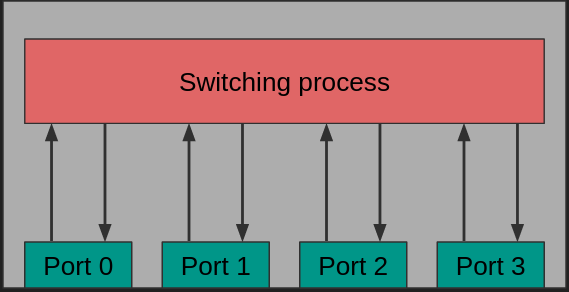
\includegraphics[width=\textwidth]{images/high-level-switch.png}
		\caption{High level overview of a network switch}
	\end{subfigure}
	\hfill
	\begin{subfigure}[b]{0.48\textwidth}
		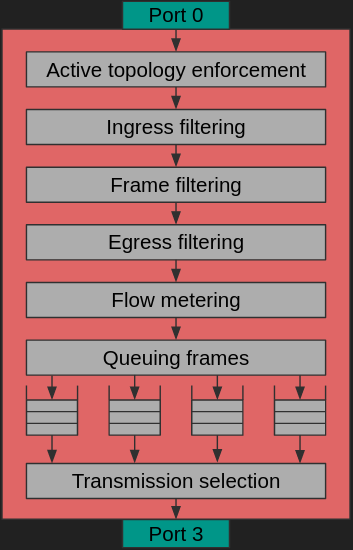
\includegraphics[width=\textwidth]{images/switching-process.png}
		\caption{Internal view of the switching process as specified in clause 8.6 of IEEE 802.1Q-2018}
	\end{subfigure}
	
	\caption{Model of a (TSN) switch showing the steps an Ethernet Frame undergoes between input and output port. Port 0 - Port 4 represent physical ports on the switch used for receiving and transmitting frames}
	\label{fig:switchinternals}
\end{figure} 
To avoid starvation of lower priority streams while still allowing prioritization an alternative \textit{Transmission selection} function has been standardized: IEEE 802.1Qav, known as the Credit Based Shaper (CBS). The Credit Based Shaper sits between a queue and the strict priority scheduler, multiple queues can have a shaper active. Each shaper acts on one specific queue only as depicted in Figure~\ref{fig:cbs}. The Credit Based Shaper limits the maximum bandwidth of a priority class by prohibiting the selection of a new frame when the allocated bandwidth has been consumed. As no frame can be selected from that priority queue, lower priority messages get the chance to be selected next. Whenever the credit of a shaper is zero or higher a frame may be selected by the strict priority scheduler. If the credit is strictly lower than zero no new frames from that queue can be selected for transmission. 
\begin{figure}[htb]
    \centering
    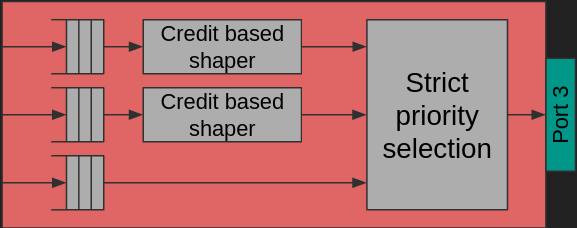
\includegraphics[width=0.6\textwidth]{images/cbs.png}
    \caption{An output port with three queues and the transmission selection implementation consisting of two credit based shapers and a strict priority scheduler}
    \label{fig:cbs}
\end{figure}

Credit of a specific shaper starts of at zero and decreases during the transmission of frames from that queue at a rate called the \textit{sendSlope}. When the credit becomes negative no new frames can be transmitted and the credit increases with a rate called the \textit{idleSlope} until it reaches zero. If the queue contains messages that are being blocked credit rises at the \textit{idleSlope} rate. Positive credit is reset to zero if the queue contains no more frames.

The CBS adds fairness and smooths out traffic bursts by limiting the bandwidth of a specific traffic class, but the total delay over multiple hops can become too large for certain control applications. IEEE 802.1Qbv, sometimes called the Time Aware Shaper (TAS) introduces a Stream Reservation Class CDT for time critical data which specifies a low worst-case latency. The TAS uses a time-division multiple access (TDMA) scheme to define a cyclic network schedule, called the gate control list. The schedule splits the network bandwidth up into time slices and defines which of the Ethernet priorities are allowed to transmit on the network during that time slice. A gate between the queue output and the priority scheduler entry opens or closes to allow or block frames to be selected by the scheduler. If two or more priorities have access to the network at the same time and have messages ready for transmission the normal strict priority scheduler decides the transmission order. An entry in the gate control list defines the state (open/closed) each gate should switch to at a specific time. The Time Aware Shaper can be used to avoid large buffering effects in the switches and removes non-deterministic interruptions by non-real time traffic.

Other shapers exist such as the IEEE 802.1Qcr Asynchronous Traffic Shaper and IEEE 802.1Qch Cyclic Queuing and Forwarding standards. Each working differently and solving a specific problem. The last relevant standards for bounded low latency are the related standards IEEE802.3br and IEEE802.1Qbu which together allow lower priority frames to be preempted during their transmission for the transmission of higher priority frames. The smallest transmittable chunk is still 64 bytes, so the high priority frames will still experience some delay.

\paragraph{Reliable frame transmission} In certain applications it is critical that messages are received without errors in their content. Ethernet protects the frame data by appending a cyclic redundancy check (CRC) and requiring a frame to be dropped when the CRC does not match the received date. Other reasons that a frame is not received can be: switch queues overflowing and hardware failure of connectors or cables. The IEEE 802.1CB standard duplicates frames and sends them over multiple disjoint paths to increase the chance that a frame arrives at the destination. The first duplicate which arrives at the destination and passes the CRC check is considered correct, the remaining frames will be discarded upon reception. If a node does not implement IEEE 802.1CB the closest IEEE 802.1CB aware switch will transparently duplicate/eliminate the frames. In an automotive setting one could imagine two disjoint paths on either side of the vehicle to increase the reliability of the network by placing the redundant paths physically far apart. 

In conclusion there is not one type of TSN network, TSN is a set of different standards trying to solve different problems in one or more ways. Depending on the requirements several TSN standards can be combined to create an Ethernet based network that is capable of reliable, time deterministic and low latency transmission of Ethernet frames. For example the Credit Based Shaper can be used together with the Time Aware Shaper to mix hard, soft and non-real time data in a single network. Which then uses IEEE 802.1CB to reliably deliver the frames over two disjoint paths.

	\section{Problem statement}

	\section{State-of-the-art analysis}
	\section{Research description}
\subsection{Research question}

\subsection{Research output}

\subsection{Development approach}

\subsection{Risks}
	\section{Feasibility experiments}
	\section{Planning}
The project has a duration of 6 months i.e 26 weeks and starts after the approval of the preparation phase, of which this document is the result.

\begin{table}[htb]
	\centering
	\begin{tabular}{cl}
		\hline
		\textbf{Week} 	& \textbf{Task} \\
		\hline
						& \textbf{Task 1} \\
		1 - 10			& subtask 1 \\
		1 - 10			& subtask n \\
		\hline
	\end{tabular}
	\caption{Planning}
	\label{tab:planning}
\end{table}
	\newpage
	\printbibliography
\end{document}